\documentclass[a4paper, 12pt, diplomski]{etf}

\usepackage{cmsrb}
\usepackage[OT2,T1]{fontenc}

\usepackage[intlimits]{amsmath}
\usepackage{amsmath, amsfonts, amssymb, graphicx}
\usepackage{cite}
\usepackage{xcolor}
\usepackage[margin=1in]{geometry}

\usepackage{icomma}
%\usepackage{upgreek}

\usepackage{mathrsfs}

\usepackage{float}


\usepackage[
    type={CC},
    modifier={by-sa},
    version={4.0},
]{doclicense}

%%%% XELATEX

\usepackage{fontspec}
\usepackage{indentfirst}
%\usepackage[margin = 0.5in]{geometry}
%\usepackage[margin=1in]{geometry}
\usepackage{titletoc}
\usepackage[Symbolsmallscale]{upgreek}
\usepackage[serbian]{babel}
\usepackage{amsmath}
\usepackage{amssymb}
\usepackage{siunitx}
\usepackage{subcaption}
\usepackage{graphicx}
\usepackage{icomma}
\usepackage{cancel}
\usepackage{physics}
\usepackage{tikz}
\usepackage{environ}
\usepackage[thinc]{esdiff}
\everymath{\displaystyle}
\usepackage{listings}
\usepackage{url}
\usepackage{xcolor}
 	\usepackage{enumerate}
\usepackage[bottom]{footmisc}

\usepackage{setspace}
\doublespacing

\setcounter{tocdepth}{3}
\setcounter{secnumdepth}{3}

\definecolor{codegreen}{rgb}{0,0.6,0}
\definecolor{codegray}{rgb}{0.5,0.5,0.5}
\definecolor{codepurple}{rgb}{0.58,0,0.82}
\definecolor{backcolour}{rgb}{0.95,0.95,0.92}
\definecolor{pythonC0}{HTML}{1F77B4} 
\definecolor{pythonC1}{HTML}{FF7F0E} 

\lstdefinestyle{mystyle}{
    backgroundcolor=\color{backcolour},   
    commentstyle=\color{codegreen},
    keywordstyle=\color{magenta},
    numberstyle=\tiny\color{codegray},
    stringstyle=\color{codepurple},
    basicstyle=\ttfamily\footnotesize,
    breakatwhitespace=false,         
    breaklines=true,                 
    captionpos=b,                    
    keepspaces=true,                 
    numbers=left,                    
    numbersep=5pt,                  
    showspaces=false,                
    showstringspaces=false,
    showtabs=false,                  
    tabsize=2
}

\lstset{style=mystyle}

\usepackage{etoolbox}
\patchcmd{\thebibliography}{\chapter*}{\section*}{}{}

\addto{\captionsserbian}{%
  \renewcommand{\bibname}{Literatura}
}

\usepackage{accents}
%\newcommand{\ul}[1]{\underaccent{\bar}{#1}}
\newcommand{\ubar}[1]{\mkern3mu\underline{\mkern-3mu #1\mkern-3mu}\mkern3mu}

\usepackage{mathtools}
%\newcommand{\ubar}[1]{\mathrlap{\underline{\vphantom{#1}\hphantom{\textup{#1}}}}#1}

\righthyphenmin1
\lefthyphenmin1

\newcommand{\navod}[1]{„#1“}
\renewcommand{\unit}[1]{\,{\rm #1}}   %-----------------
%\usepackage{mathptmx}
%\setmainfont{Times New Roman}'
\newcommand{\DS}{\displaystyle}
%\newcommand{\faz}[1]{\underbar{#1}}

\usepackage{accents}
\newcommand{\faz}[1]{\underaccent{\bar}{#1}}

%%%

%\title{
%Implementacija i postupak kalibracije skalarnog analizatora %mreža 
%u opsegu mikrotalasnih učestanosti 300\,MHz -- 3\,GHz
%}
%\author{Danilo Đokić}
%\indeks{2016/0116}
%\date{Septembar 2020.}
%\mentor{doc. dr Slobodan Savić}
%\predmet{}

\frenchspacing

\begin{document}

%\fontencoding{OT2}\selectfont

%\maketitle

\begin{center}
    {
    \Large
    \textsc{Univerzitet u Beogradu} \\
    \textsc{Elektrotehnički fakultet} \\
	
	\vspace{22pt}    
    
    %
\includegraphics[scale=.5]{fig/etf-logo-lat.jpg}
    
\includegraphics[scale=.5]{fig/etf_logo.png}
    
    \vfill
    
    \LARGE
    Upravljanje brzinom motora jednosmerne struje primenom analogne negativne povratne sprege
    } \\[2mm]
    {\large Diplomski rad}
    
    \vfill
    
    \large 
    
    \begin{minipage}[t]{.49\textwidth}
    \begin{flushleft}    
    Mentor:     \\
    Dr Radivoje Đurić, \\
    vanredni profesor
    \end{flushleft}
    \end{minipage}
    \begin{minipage}[t]{.49\textwidth}
    \begin{flushright}
    Kandidat: \\
    David Milovanović, 2016/0274
    \end{flushright}
    \end{minipage}

    
    \vfill
    
    Beograd, Septembar 2022.
\end{center}

\thispagestyle{empty}

\newpage

\tableofcontents

\begingroup
\let\clearpage\relax
\listoffigures
\endgroup

\newpage

%\begin{abstract}
%\end{abstract}

%\begin{keywords}
%\end{keywords}

%\tableofcontents
%\listoffigures
%\listoftables

\newpage

\begin{center}
\vspace*{\fill}

	\begin{Large}
		\textbf{Zahvalnica}
	\end{Large}
	
	Zahvaljujem se svima koji su doprineli izradi ovog diplomskog rada, a posebno svom mentoru Dr Radivoju Đuriću, vanrednom profesoru koji je omogućio izradu teme ovog diplomskog rada i Ms Danilu Đokiću, asistentu koji je omogućio konstantnu podršku tokom izrade ovog rada.
	
	Najveću zahvalnost za bezgraničnu podršku tokom studiranja i izrade diplomskog rada, dugujem svom ocu Zoranu Milovanoviću.
	
	\hfill Iskreno vam hvala.\\
	\hfill David Milovanović
		
\vspace*{\fill}	
\end{center}

\begin{abstract}
	
	Jednosmerni motor je veoma zastupljen u sferama gde postoji neka vrsta upravljanja sistema. U ovom radu će biti uvedeni i objašnjeni osnovni principi funkcionisanja analognog sistema upravljanja motora jednosmerne struje. Takođe, biće isprojektovan sistem i izvršena sva potrebna merenja i njihova obrada, i izvršiće se poređenje izmerenih rezultata sa očekivanim teorijskim rezultatima.
	
	Rad je organizovan u tri odeljka. U teorijskom uvodu su uvedeni opšti pojmovi koji predstavljaju delove sistema koji se projektuje. Dodatno, u ovom delu su date i teorijske predikcije ponašanja sistema. U odeljku \navod{Karakteristike korišćenih komponenti} su opisane karakteristike korišćenih delova sistema i data su merenja njihovih osobina koja su značajna za dalje modifikacije sistema. U odeljku \navod{Rezultati i diskusija} su navedeni rezultati celog sistema kao i ocena njihovog preklapanja sa očekivanim teorijskim rezultatima koji su dobijeni ranije.
    
	Cilj rada je da je moguće isprojektovati analogni sistem upravljanja koji će davati relativno iste rezultate kao i teorijski model sistema. U radu je pokazano da se uz pomoć teorije mogu dobiti parametri kontrolera sistema koji će i praktično davati iste rezultate kao i teorijski.     
 \\[10mm]
    
    \doclicenseThis
    
    \vspace{1mm}
     
    
    Online repozitorijum sa izvornim kodovima dostupan je
    na \url{https://github.com/dejvi997}.
\end{abstract}


\newpage

\section{Teorijski uvod}
\subsection{Analogni sistemi automatskog upravljanja}
Sistem automatskog upravljanja predstavlja sklop električnih i mehaničkih elemenata koji vrši funkcije koje su im zadate kontrolnim signalima, na kontrolisan način, između ostalog, uz obezbeđivanje povratne informacije o stanjima delova sistema od interesa. Primer nekih od funkcija koje se mogu vršiti su kontrola izlaznog napona, održavanje stalne brzine okretanja osovine, podešavanje temperature itd. Postoje dve veće grupe sistema automatskog upravljanja, analogni i digitalni. 
Digitalni sistemi automatskog upravljanja koriste digitalne računare u ulozi kompenzatora i regulatora. Oni koriste digitalne odnosno numeričke podatke tako što se analogna merena veličina uz pomoć AD konvertora pretvori u digitalni domen, zatim digitalni računar obradi podatke i da na svom izlazu takođe digitalni podatak koji se dalje vodi na DA konvertor kako bi se signal vratio u analogni domen, i onda se dalje prosleđuje sistemu kojim se upravlja. S druge strane, analogni sistemi upravljanja rade sa kontinualnim signalima, i nemaju problema gubitka informacija usled konačne preciznosti AD i DA konvertora. Takođe, podaci se ne obrađuju na svaku periodu takta nego kontinualno i izlaz sistema za kontrolu je takođe analogni signal. Još jedna prednost analognih sistema je njihova robusnost, naime, ako dođe do male promene napona usled neke greške, to neće mnogo uticati na konačni rezultat, dok kod digitalnih sistema to može dovesti do prebacivanja napona iznad ili ispod nekog od praga odlučivanja i pri daljoj obradi se može desiti da se napravi veća greška. Konkretan cilj ovog rada jeste projektovanje analognog sistema automatskog upravljanja uz pomoć kojeg bi se kontrolisao motor jednosmerne struje. Dodatno, uz pomoć povratne sprege bi se održavala zadata brzina motora bez obzira na to na koliki otpor nailazi osovina motora, odnosno obezbeđuje se imunost na poremećaj.

\subsection{Motor stalne struje}
\subsubsection{Princip funkcionisanja}

Jednosmerni motor je električna mašina koja pretvara električnu energiju u mehaničku, uz korišćenje jednosmerne struje, na osnovu čega se svrstava u pretvarače elektromehaničke energije. Konstrukcijski deo jednosmernog motora se sastoji iz dva dela, statora i rotora. Stator obezbeđuje konstantno magnetsko polje, dok kroz rotor protiče jednosmerna struja koja indukuje elektromagnetsko polje, i pri proticanju struje kroz namotaje rotora koji se nalaze u konstantnom polju, javlja se pokretački moment koji okreće rotor. Svi relevantni efekti za projektovanje i analizu sistema upravljanja motora stalne struje se mogu dobiti iz pojednostavljenog modela sistema koji je prikazan na slici \ref{blokDC}.

\begin{figure}[h!]
    \centering
    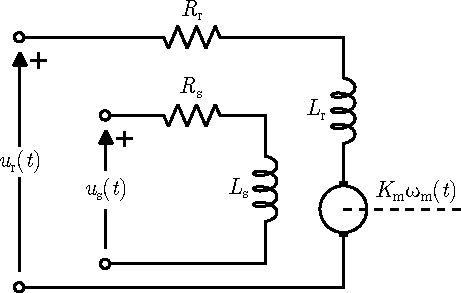
\includegraphics[scale=1]{fig/DCmotor.pdf}
    \caption{Principska šema jednosmernog motora.}
    \label{blokDC}
\end{figure}

\noindent
Od interesa je veza između ugaone brzine motora $\upomega_{\rm m}(t)$ i napona na rotoru $v_{\rm r}(t)$, odnosno prenosna funkcija $G(s) = \frac{\Omega_{\rm m}(s)}{V_{\rm m}(s)}$ koja se može aproksimirati sistemom prvog reda kao:

\begin{equation}
	G(s) = \frac{K_{\rm m}}{T_{\rm m}s+1}\:.
	\label{eq:prenosnaDC}
\end{equation}

\noindent
Konstanta $K_{\rm m}$ predstavlja statičko pojačanje, dok konstanta $T_{\rm m}$ predstavlja vremensku konstantu jednosmernog motora upravljanog strujom u rotoru. \cite{osuDC}

\break

\subsubsection{Odskočni odziv}

Poznavanje odziva sistema na odskočnu pobudu je značajno za predikciju ponašanja sistema na različite pobude, jer se na osnovu toga može predvideti ponašanje odziva sistema za proizvoljnu pobudu. 
Ako je poznat odskočni odziv sistema, tada se na osnovu toga mogu odrediti neki od parametra posmatranog sistema i njegove osobine.
Što znači, ako ulazni signal predstavlja odskočnu pobudu: $v_{\rm U}(t) = V_0u(t)$, primenom Laplasove transformacije signal se prebacuje u kompleksni domen kao: $V_{\rm U}(s) = \mathscr{L}\{ v_{\rm U}(t) \} = \frac{V_0}{s}$.
Ako se za model sistema koristi uprošćeni model dat u izrazu \eqref{eq:prenosnaDC}, odziv na odskočnu pobudu, u kompleksnom domenu, se  dobija kao:
$V_{\rm I}(s) = G(s) V_{\rm U}(s)$, što je u vremenskom domenu dato izrazom: $v_{\rm I}(t) = V_0K_{\rm m}\left(1 - \exp \left( - \dfrac{t}{T_{\rm m}}  \right) \right) $. Na slici \ref{DCmodel} su prikazani grafici sa različitim vrednostima parametra radi ilustracije ponašanja modela motora. Dodatno na slici \ref{DCmodel} konstanta $V_{\rm k}$ je bezdimenziona i data je relacijom $V_{\rm k} = \frac{V_0K_{\rm m}}{1\unit{V}}$.


\begin{figure}[h!]
    \centering
    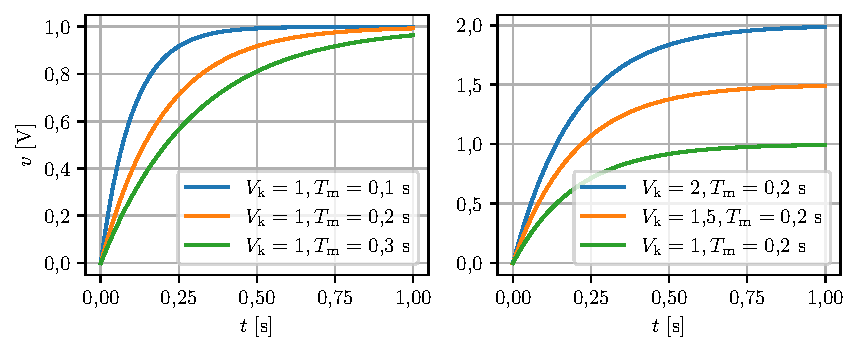
\includegraphics[scale=1]{fig_teorija/DCmodeli.pdf}
    \caption{Modelovana karakteristika jednosmernog motora.}
    \label{DCmodel}
\end{figure}


\subsection{Rotacioni enkoder}
\subsubsection{Princip funkcionisanja} \label{sec:PrincipFunkcionisanja}
Uloga enkodera je da obezbeđuje informaciju o trenutnom položaju, odnosno smeru okretanja osovine. Enkoder je sačinjen iz diska priključenog za osovinu rotora, i na sebi ima proreze kroz koje može da prođe svetlost. S jedne strane je optički uređaj koji emituje svetlosne zrake dok je s druge strane optički uređaj koji ih prima. Ako se taj svetlosni signal prevede u električni, imaće oblik povorke pravougaonih impulsa. Dodatno, ako enkoder ima opciju da daje informaciju o smeru, jedna od implementacija je da se ispod postojećih proreza nalazi još jedan set proreza koji je celokupno pomeren u jednu stranu u odnosu na proreze iznad. 
Na taj način se dobijaju dva signala, signal \navod{u fazi} i signal \navod{u kvadraturi}, od kojih je jedan fazno pomeren u vremenu. U odnosu na to koji od signala prednjači, može se jednoznačno imati informacija o smeru kretanja. Na slici \ref{enc} je ilustrativno pokazan princip rada enkodera.


\begin{figure}[h!]
    \centering
    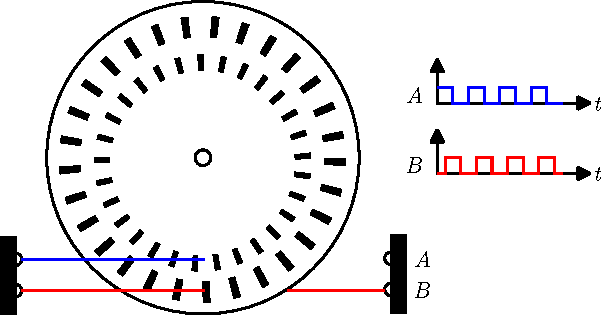
\includegraphics[scale=1]{fig/enc.pdf}
    \caption{Enkoder.}
    \label{enc}
\end{figure}


Konačno, ako se zna broj proreza na enkoderu može se odrediti i ugaona brzina motora $\upomega_{\rm m}$ uz minimalnu grešku koja se svodi na preciznost merenja. U ovom radu je korišćen motor stalne struje sa ugrađenim enkoderom koji radi na ovom principu. Radi jednostavnosti, u ovom radu razmatra se upravljanje brzine motora bez promene smera okretanja, na osnovu čega se koristi samo jedan signal.


\subsubsection{Pretvarač učestanosti u napon} \label{s:fv} \label{sec:fvKonvertor}

Kao što je već pomenuto u delu \ref{sec:PrincipFunkcionisanja}, izlazni signal enkodera je oblika povorke pravougaonih impulsa čija je frekvencija srazmerna brzini okretanja osovine. Pošto u analognom sistemu automatskog upravljanja signal treba da bude srazmeran merenoj veličini, potrebno je isprojektovati konvertor koji će od signala koji se dobija sa enkodera, koji predstavlja signal sa promenljivom učestanošću, dati signal koji predstavlja signal sa promenljivim nivoom. Šema konvertora je data na slici \ref{fvKonvertor}.

\break

\begin{figure}[h!]
    \centering
    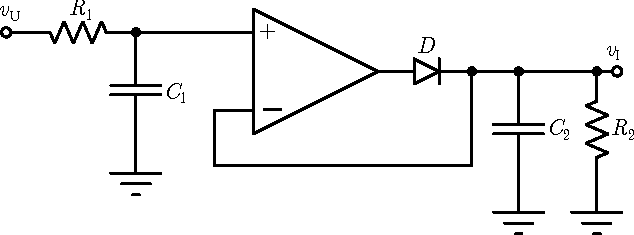
\includegraphics[scale=1]{fig/fvKonvertor.pdf}
    \caption{Pretvarač frekvencije u napon.}
    \label{fvKonvertor}
\end{figure}

Na ulazu u pretvarač se nalazi filtar propusnik niskih učestanosti čija je uloga da na svom izlazu da signal čija je amplituda zavisna od učestanosti ulaznog signala. $R_1$ i $C_1$ se biraju tako da je vremenska konstanta filtra manja od periode ulaznog signala, kako bi filtar mogao da isprati svaku periodu. Signal se dalje vodi na precizni usmerač i paralelnu vezu otpornika i kondenzatora, koji zajedno čine detektor anvelope amplitude u nivo. Drugi par $R_2C_2$ na izlazu se biraju da njihova vremenska konstanta bude veća kako bi držali nivo signala na izlazu dovoljno dugo dok ne dođe informacija o sledećoj periodi iz prethodnog dela kola.

Dodatno, u signalu na izlazu konvertora se javlja veliki šum zbog vremenske $R_1C_1$ konstante koja je potrebno da bude mala kako bi kolo ispratilo dinamiku signala ali zbog toga se pojačava šum u zonama konstantnog signala. Taj šum zavisi od ulaznog $R_1C_1$ filtra, što je vremenska konstanta veća frekvencija šuma će biti manja ali amplituda veća, dok će sa manjom vremenskom konstantom biti dualno.

\subsubsection{Pretvarač učestanosti u napon sa NF filtrom} \label{s:FVNF}

Da bi se problem uveden u prethodnoj tački rešio, signal se može propustiti kroz filtar propusnik niskih učestanosti. Potrebno je izabrati takvu graničnu učestanost filtra kako bi se filtrirao šum koji je posledica pretvarača, a očuvala brzina promene nivoa signala. 
Konvertor iz tačke \ref{sec:fvKonvertor} će dati relativno konstantan napon za konstantne brzine motora ali usled velike učestanosti signala na izlazu enkodera će se javiti šum. Radi smanjenja snage šuma, signal se propušta kroz filtar propusnik niskih učestanosti.
Filtar koji se može iskoristiti je pasivan $RC$ filtar čija je šema prikazana na slici \ref{NFfiltar} a prenosna karakteristika na slici \ref{NFprenosna}. Granična učestanost predstavlja učestanost na koju fazna karakteristika filtra opadne za $45^{\circ}$, i ona se računa kao: $f_{\rm{gr}} = \frac{1}{2 \pi RC}$. Podešavanjem vrednosti za $R$ i $C$ može se podešavati granična učestanost, takva da omogući da filtar oslabi šum na većim učestanostima, a propusti učestanosti na kojima se menja nivo signala. Za konvertor će se u nastavku podrazumevati konvertor sa NF filtrom.
Ovaj konvertor se u sistemu koji opisujemo predstavlja kao blok prenosne funkcije $F(s)$ u izrazu \eqref{eq:nps}.

\begin{center}
\begin{minipage}{0.5\textwidth}
\centering
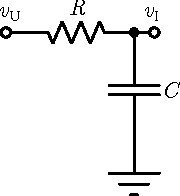
\includegraphics[scale=1]{fig/NF.pdf}
\captionof{figure}{Šema NF filra}
\label{NFfiltar}
\end{minipage}%\hfill
\begin{minipage}{0.5\textwidth}
\centering
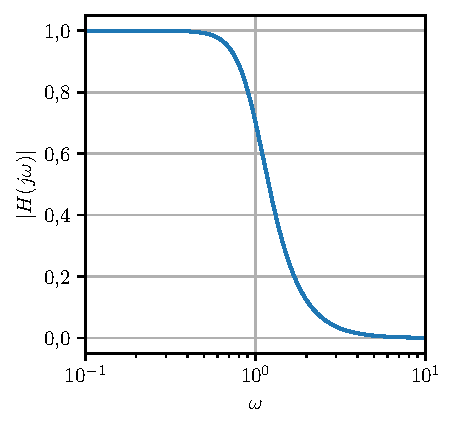
\includegraphics[scale=1]{fig_teorija/NFkka.pdf} 
\captionof{figure}{Prenosna karakteristika NF filtra.}  
\label{NFprenosna} 
\end{minipage}
\end{center}


\subsection{Princip negativne povratne sprege}

Negativna povratna sprega se javlja kada se neka funkcija izlaza sistema, procesa ili mehanizma dovede \navod{nazad} na ulaz na taj način da smanjuje fluktuacije izlaza, koje su posledice promene ulaznog signala ili smetnji. Opšta blok šema sistema sa negativnom povratnom spregom je data na slici \ref{nps}.

\begin{figure}[h!]
    \centering
    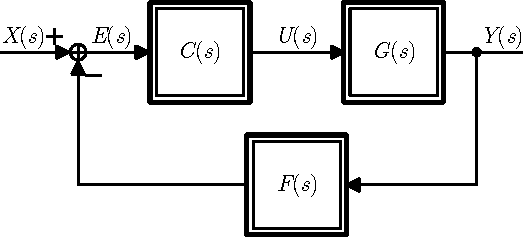
\includegraphics[scale=1]{fig/nps.pdf}
    \caption{Opšta struktura sistema sa negativnom povratnom spregom.}
    \label{nps}
\end{figure}

Signal $E(s)$ predstavlja signal greške za koji je u idealnom slučaju trebao da bude nula u svakom trenutku, ali pri promeni ulaznog napona usled realne dinamike sistema se javlja signal greške i on služi da kontroleru da informaciju kolika je greška kako bi kontroler mogao da dovede sistem u željeno stanje. Dobijeni signal greške nam govori koliko je odstupanje i kako dalje treba da se upravlja sistem da bi se dobio željeni rezultat. Signal greške $E(s) = X(s) - F(s)Y(s)$ nakon prolaska kroz kontroler daje signal $U(s)$ koji predstavlja upravljački signal koji se generiše u odnosu na signal greške $E(s)$ i prenosne funkcije upravljačkog bloka $C(s)$, kao  $U(s) = E(s)C(s)$. On se dalje dovodi na ulaz pogonskog bloka predstavljenog prenosnom funkcijom $G(s)$.
Prenosna funkcija celokupnog sistema od ulaznog signala, do izlaza je $W(s)$ i određena je izrazom:

\begin{equation}
	W(s) = \frac{C(s)G(s)}{1 + F(s)C(s)G(s)}.
	\label{eq:nps}
\end{equation}



\subsection{Regulatori}

\subsubsection{\textit{Bang-bang} regulator} \label{s:bangbang}

Uloga regulatora u sistemu jeste da kontroliše, odnosno reguliše sistem tako da se ostvari željeno ponašanje. Konkretno, P kontroler ili proporcionalni kontroler radi po principu množenja konstantom. Naime, signal greške se množi konstantom kako bi se prividno greška povećala što dalje dovodi do burnije reakcije sistema na ispravljanje te greške. Problem koji može da se javi prilikom korišćenja ovog kontrolera jesu preskoci u izlaznom signalu koji vremenom prelaze u oscilacije i uzrokuju nestabilnost sistema. Konstanta kojom se množi signal greške se drugačije zove pojačanje i njegovim menjanjem može da se menja i \navod{burnost} odziva sistema.
U ovom radu su korišćeni \textit{Bang-bang}, P i PI regulatori. U ovoj tački se posmatra \textit{Bang-bang} regulator koga karakteriše pojačanje koje teži beskonačnosti. Beskonačno pojačanje je realizovano idealnim operacionim pojačavačem. 


Dodatno, ovaj element spada u grupu kontrolera i on se u sistemu koji opisujemo predstavlja kao blok prenosne funkcije $C(s)$ u principskoj jednačini \eqref{eq:nps}.
Performanse P regulatora zavise od njegovog pojačanja. U konkretnom slučaju pojačanje teži beskonačnosti, i ako se to uvrsti u jednačinu \eqref{eq:nps}, znajući da je $C(s) = K_{\rm p}$, čak i neznajući ostale funkcije, dobija se: $W(s) = \lim_{C(s) \to \infty} \frac{C(s)G(s)}{1 + F(s)C(s)G(s)} =$ \navod{ $\frac{\infty}{1 + \infty}$ } $ = 1$.


\subsubsection{P regulator}

U delu \ref{s:bangbang} je pomenuta jedna varijanta P regulatora, koji ima beskonačno pojačanje i oscilacije u stacionarnom stanju. Da bi se rešio problem sa oscilacijama potrebno je smanjiti pojačanje na neku realnu vrednost koja nije beskonačna. Time se dobija P regulator koji nema oscilacije u stacionarnom stanju ali i dalje ostaje konačna greška u stacionarnom stanju. Opšta blok šema sa \textit{bang-bang}, odnosno P regulatorom je prikazana na slici \ref{Preg}.


\begin{figure}[h!]
    \centering
    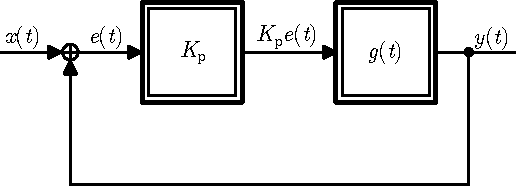
\includegraphics[scale=1]{fig/Preg.pdf}
    \caption{Blok šema sistema sa $\Pi$ regulatorom.}
    \label{Preg}
\end{figure}



\subsubsection{PI regulator} \label{s:PI}

Kod sistema sa P regulatorom se javlja problem konstantne statičke greške, a zbog prevelikog pojačanja može doći do oscilovanja izlaza jer će sistem pojačati šum što realne komponente \navod{otera} u zasićenje. Rešenje je dodavanje integratora koji se ponaša kao filtar propusnik niskih učestanosti i koji će obezbediti nultu grešku u stacionarnom stanju, i potencijalno ubrzati sistem uz dodavanje određenog procenta preskoka. Prenosna funkcija integratora je oblika $\frac{1}{T_{\rm i}s}$, gde je $T_{\rm i}$ vremenska konstanta integratora. Znajući da je prenosna funkcija za P kontroler konstanta, za PI regulator se dobija izraz $K_{\rm p} + \frac{1}{T_{\rm i}s}$. Blok šema realizacije PI regulatora je prikazana na slici \ref{PIreg}.


\begin{figure}[h!]
    \centering
    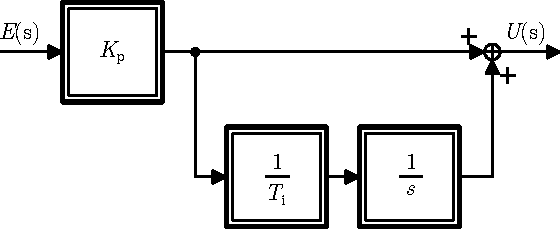
\includegraphics[scale=1]{fig/PIreg.pdf}
    \caption{Blok šema PI regulatora.}
    \label{PIreg}
\end{figure}

Dodatno, poznavanjem modela sistema kojim se upravlja, se može u nekom od softverskih alata napraviti model PI regulatora i na taj način uštedeti vreme projektovanja regulatora sa optimalnim konstantama. Način određivanja konstanti regulatora je iterativan postupak, jer se ne može generalizovati nego zavisi od toga šta je optimalno za dati problem i samog sistema, odnosno njegove osetljivosti na preskoke i brze pobude.
Ako se modifikuje blok šema sa slike \ref{nps} tako da izgleda kao na slici \ref{nps2}, može se izvesti izraz za funkciju spregnutog prenosa $W(s)$. Imajući u vidu brzu dinamiku pretvarača onda važi da je prenosna funkcija sistema bez kontrolera $H(s) = G(s)F(s) = \frac{K_{\rm m}}{T_{\rm m}s + 1}$, znajući da za PI kontroler važi $C(s) = K_{\rm p} + \frac{1}{T_{\rm i}s}$, ako se to uvrsti u jednačinu \eqref{eq:nps}, dobija se $W(s) = \frac{\left( K_{\rm p} + \frac{1}{T_{\rm i}s} \right) \frac{K_{\rm m}}{T_{\rm m}s + 1} }{ 1 + \left( K_{\rm p} + \frac{1}{T_{\rm i}s} \right) \frac{K_{\rm m}}{T_{\rm m}s + 1} }$. \cite{osuREG}

\begin{figure}[h!]
    \centering
    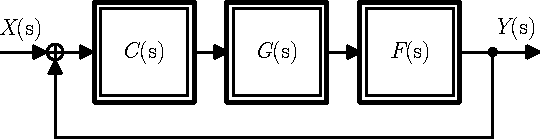
\includegraphics[scale=1]{fig/nps2.pdf}
    \caption{Blok šema sistema sa PI regulatorom sa jediničnom povratnom spregom.}
    \label{nps2}
\end{figure}


\subsection{Pojačavač snage}
\subsubsection{Pojačavač snage u klasi B} \label{s:PAB}

Pojačavač snage u klasi B je pojačavač koji ima pojačanje 1 i potencijalno \textit{crossover} izobličenja, električna šema je prikazana na slici \ref{PAb}. Izobličenja se mogu bolje videti na prenosnoj karakteristici na slici \ref{PAbkka} gde je prikazan izlazni napon $v_{\rm i}(t)$ u funkciji ulaznog napona $v_{\rm u}(t)$.


\begin{center}
\begin{minipage}{0.5\textwidth}
\centering
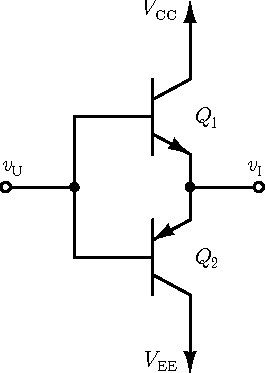
\includegraphics[scale=1]{fig/PAB.pdf}
\captionof{figure}{Pojačavač snage u klasi B.}
\label{PAb}
\end{minipage}%\hfill
\begin{minipage}{0.5\textwidth}
\centering
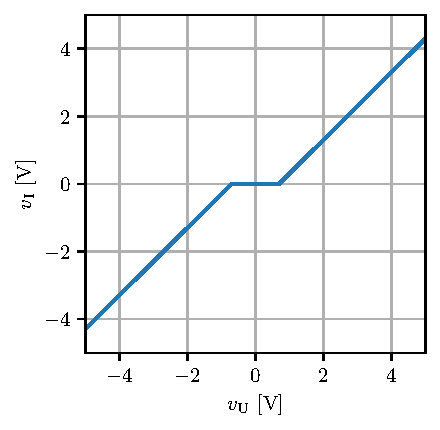
\includegraphics[scale=1]{fig_teorija/PAbkka.pdf} 
\captionof{figure}{Prenosna karakteristika pojačavača u klasi B, za napon $|V_{\rm B \rm E}| = 0.7 \rm V$.}  
\label{PAbkka} 
\end{minipage}
\end{center}

Za pozitivne vrednosti ulaznog napona veće od napona $|V_{\rm B \rm E}|$, pnp tranzistor je zakočen, dok npn tranzistor radi u direktnom aktivnom režimu. Dok za negativne vrednosti ulaznog napona važi dualno, kada je ulazni napon manji od $-|V_{\rm B \rm E}|$, npn tranzistor je zakočen, dok pnp tranzistor radi u direktnom aktivnom režimu. Dok je u oblasti ulaznog napona između $-|V_{\rm B \rm E}|$ i $|V_{\rm B \rm E}|$ izlaz jednak nuli, u slučaju simetričnog napajanja. Vremenski dijagram jedne periode ulaznog i izlaznog signala na pojačavaču je ilustrovan na slici \ref{vremenskiPAb}


\begin{figure}[!h]
    \centering
    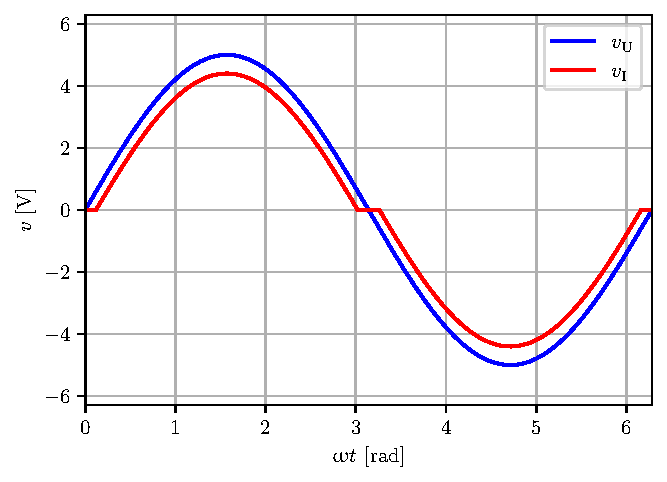
\includegraphics[scale=1]{fig_teorija/crossover.pdf}
    \caption{Vremenski dijagram ulaznog i izlaznog signala.}
    \label{vremenskiPAb}
\end{figure}


\break

\subsubsection{Pojačavač snage u klasi B sa negativnom povratnom spregom} \label{s:PAB}

Pošto je za pokretanje motora potrebna velika snaga, samo povezivanje kontrolnog napona sa generatora signala na motor ne bi bila dovoljna jer bi motor \navod{povukao} dosta struje, i zbog toga se ubacuje pojačavač snage, ali i povratna sprega kako bi postojala informacija uz pomoć koje je moguće kontrolisati motor. 

\begin{figure}[h!]
    \centering
    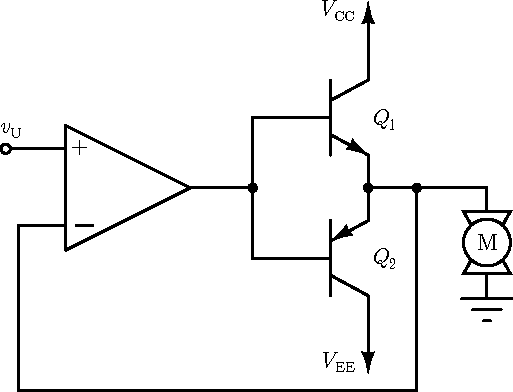
\includegraphics[scale=1]{fig/PABnps.pdf}
    \caption{Pojačavač snage u klasi B sa negativnom povratnom spregom.}
    \label{PAbNPS}
\end{figure}


\subsubsection{Pojačavač snage u klasi AB sa negativnom povratnom spregom} \label{s:PAAB}

Problem koji se ovde javlja kod pojačavača u klasi B je \textit{crossover} izobličenje zbog kojeg se ne može imati napon na izlazu veći od $V_{\rm{CC}} - |V_{\rm B \rm E}|$, odnosno manji od $V_{\rm{EE}} + |V_{\rm B \rm E}|$ i zone ulaznog signala koji je u opsegu od $-|V_{\rm B \rm E}|$ do $|V_{\rm B \rm E}|$ gde je konstantno nula na izlazu. Rešenje tog problema je modifikacija pojačavača dodavanjem dve diode sa naponom provođenja $V_{\rm D} = |V_{\rm B \rm E}|$ za polarizaciju tranzistora. Time se dobija pojačavač u klasi AB čija je šema prikazana na slici \ref{PAAB}. Teorijski, naponi praga dioda i tranzistora su jednaki, i prenosna funkcija u tom slučaju linearna i može se videti na slici \ref{PAABkka}. Problemi toga su neidealnosti realnih komponenti, odnosno razlika napona praga diode i napona napona praga tranzistora.


\begin{center}
\begin{minipage}{0.5\textwidth}
\centering
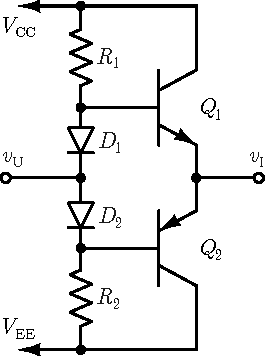
\includegraphics[scale=1]{fig/PAAB.pdf}
\captionof{figure}{Pojačavač snage u klasi AB.}
\label{PAAB}
\end{minipage}%\hfill
\begin{minipage}{0.5\textwidth}
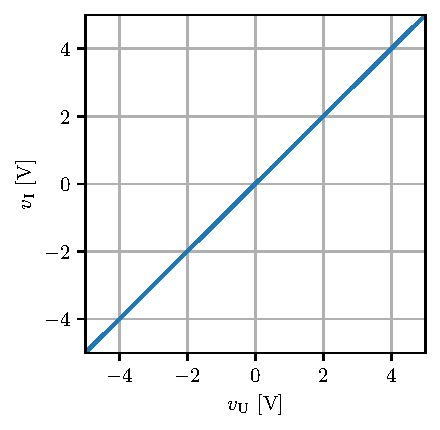
\includegraphics[scale=1]{fig_teorija/PAABkka.pdf} 
\captionof{figure}{Prenosna karakteristika pojačavača u klasi AB.}  
\label{PAABkka} 
\end{minipage}
\end{center}

\begin{figure}[h!]
    \centering
    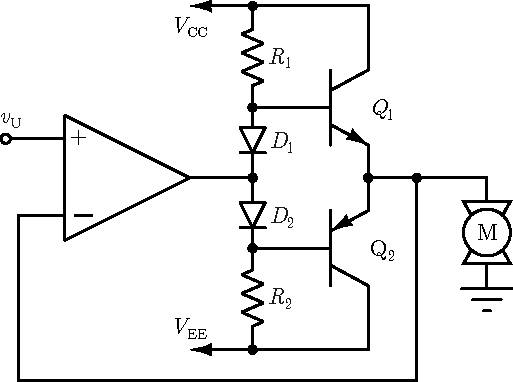
\includegraphics[scale=1]{fig/PAABnps.pdf}
    \caption{Pojačavač snage u klasi AB sa negativnom povratnom spregom.}
    \label{PAABnps}
\end{figure}

\break

\section{Karakteristike korišćenih komponenti sistema}

U ovom poglavlju, akcenat će biti na opisivanje komponenti sistema korišćenih za dobijena merenja.

\subsection{Identifikacija modela motora}

\subsubsection{Merenje odziva motora}

Šema koja je korišćena za merenje odziva jednosmernog motora je data na slici \ref{DCsema1}.

\begin{figure}[h!]
    \centering
    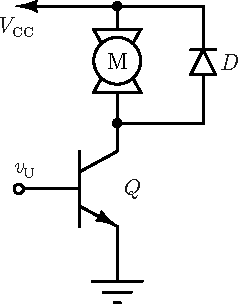
\includegraphics[scale=1]{fig/DCtransistor.pdf}
    \caption{Eksperimentalna postavka za merenje odziva jednosmernog motora.}
    \label{DCsema1}
\end{figure}

\noindent
Uz pomoć osciloskopa i računara povezanog sa osciloskopom je izmerena karakteristika jednosmernog motora na odskočnu pobudu.

\noindent
Na slici \ref{compact} je uz pomoć metode najmanjih kvadrata odrađeno modelovanje krive funkcijom oblika 
$f(t) = V_0K_{\rm m}\left(1 - \exp \left( - \dfrac{t}{T_{\rm m}}  \right) \right) $
Određivanje optimalne krive obavljeno je pomoću funkcije 
\verb|scipy.optimize.curve_fit| u programskom jeziku Python. 
Funkcija \verb|curve_fit| radi po metodi najmanjih kvadrata, odnosno, pravi model funkcije koja će imati najmanju kvadratnu grešku u odnosu na podatke koji su joj prosleđeni.
Ako su poznati izmereni odbirci odskočnog odziva sistema, tada je poznata i povezanost vrednost trenutnog odbirka izlaza sa svim prethodnim odbircima izlaza, odnosno: $v_{\rm I}[n-n_0] = f(v_{\rm I}[n - n_j]) \, , \, \forall \, n_j : \{n - n_j < n - n_0\}$.
Mora postojati inicijalna pretpostavka oblika funkcije kako bi se model estimirao na najbolji mogući način. Potrebno je imati neku informaciju o prirodi podataka koji se prosleđuju funkciji kao što su početni uslovi i parametri koji utiču na sam oblik funkcije. Osciloskop daje dobru rezoluciju signala na manjim učestanostima, dok na većim učestanostima Arduino bolje prikuplja podatke zbog konstantne velike rezolucije. Ograničenje osciloskopa potiče od konačnog broja tačaka na ekranu osciloskopa, konkretno 2500, dok je kod Arduina taj broj znatno veći, odnosno frekvencija učestanosti dobijanja merenih tačaka je $1.23$ MHz.


\begin{figure}[h!]
    \centering
    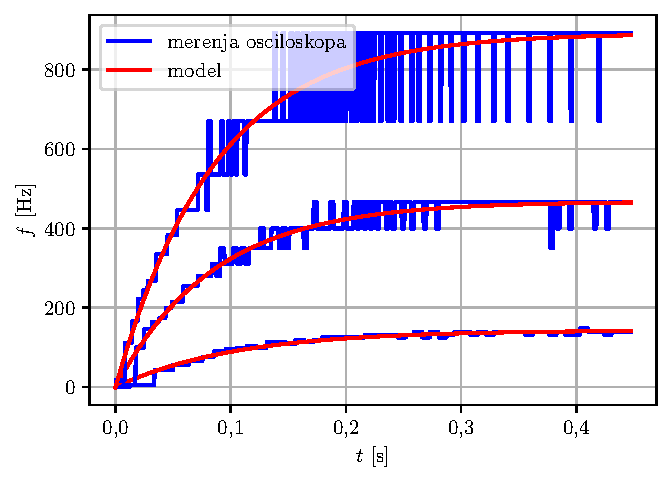
\includegraphics[scale=1]{fig_osc/compact.pdf}
    \caption{Određivanje optimalnog modela motora na osnovu merenog odskočnog odziva.}
    \label{compact}
\end{figure}

Signal koji se posmatrao na prethodnim graficima je izlazni signal enkodera motora koji je oblika povorke pravougaonih impulsa sa promenljivom frekvencijom koja je srazmerna brzini okretanja osovine jednosmernog motora.

Dodatno, parametri signala sa grafika sa slike \ref{compact} prikazani u tabeli \ref{tab:tabela1}, u sortirani u rastućem poretku granične frekvencije. \cite{oe} 
\cite{encArduino} 
\cite{curveFit}

\begin{center}
\begin{tabular}{||c |c|  c||} 
 \hline
 Br. & $K_{\rm m}$ & $T_{\rm m} [\rm s]$  \\ [0.5ex] 
 \hline\hline
 1 & 143,45 & 1,97  \\ [0.5ex]
 \hline
 2 & 468,03 & 0,57  \\ [0.5ex]
 \hline
 3 & 892,08 & 0,35  \\ [0.5ex] 
 \hline
\end{tabular}
\label{tab:tabela1}
\end{center}

\noindent


\begin{center}
\begin{minipage}{0.45\textwidth}
\centering
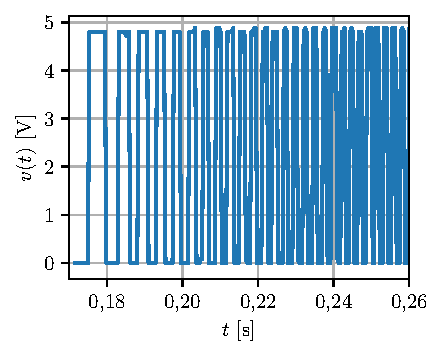
\includegraphics[scale=1]{fig_osc/vremenski.pdf}
\captionof{figure}{Vremenski oblik signala na izlazu enkodera, prilikom ubrzanja motora.}
\label{vremenski}
\end{minipage}\hfill
\begin{minipage}{0.45\textwidth}
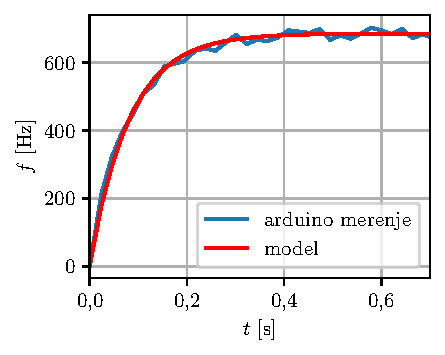
\includegraphics[scale=1]{fig_arduino/Startup670.pdf} 
\captionof{figure}{Izmerena vremenska zavisnost frekvencije signala na izlazu enkodera i model sa parametrima: $K_{\rm m} = 679$ i $T_{\rm m} = 481 \, \rm{ms}$.}  
\label{arduino670} 
\end{minipage}
\end{center}



\subsubsection{Merenje prenosne statičke karakteristike motora sa i bez filtra na izlazu}

Bez NF filtra motor kreće da ubrzava od $3.5 \unit{V}$ do $4.6 \unit{V}$. Dodatno u ovom slučaju nije korišćen precizni usmerač nego običan bafer u kolu za konvertovanje frekvencije u napon. Grafik zavisnosti nivoa izlaznog napona od nivoa ulaznog napona je prikazan na slici \ref{DCsweep}.


Pošto šum predstavlja problem, dodavanjem NF filtra se taj problem može rešiti i dobija se drugačiji rezultat, odnosno da do $3 \unit{V}$ ulaznog napona, motor ima konstantu brzinu, a onda se brzina povećava s porastom ulaznog napona. Posledica razlike napona aktivacije motora od $0.5 \unit{V}$ je pad napona na diodi u preciznom usmeraču pomenutog u delu \ref{sec:fvKonvertor}. Grafik zavisnosti nivoa izlaznog napona od nivoa ulaznog napona je prikazan na slici \ref{DCsweepNF}.

\begin{center}
\begin{minipage}{0.45\textwidth}
\centering
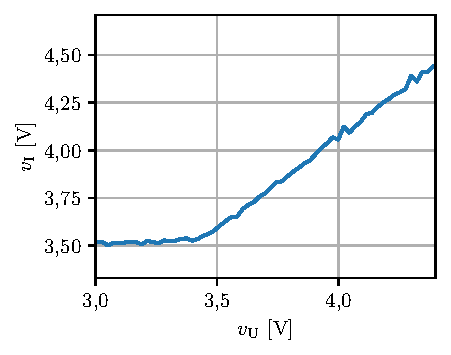
\includegraphics[scale=1]{fig_osc/DCsweep.pdf}
\captionof{figure}{Statička prenosna karakteristika celog sistema.}
\label{DCsweep}
\end{minipage}\hfill
\begin{minipage}{0.45\textwidth}
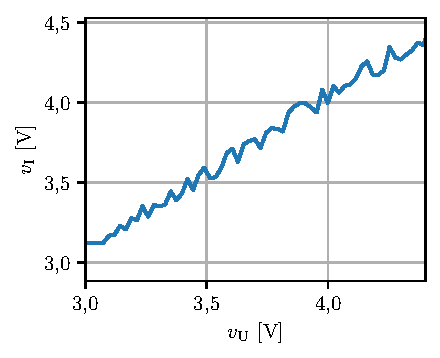
\includegraphics[scale=1]{fig_osc/DCsweepNF.pdf} 
\captionof{figure}{Statička prenosna karakteristika celog sistema sa NF filtrom.}  
\label{DCsweepNF} 
\end{minipage}
\end{center}



\subsection{Merenje karakteristika pretvarača učestanosti}
\subsubsection{Karakteristika pretvarača bez filtra}

Kao što je opisano u delu \ref{s:fv}, pretvarač bi u idealnom slučaju, za napon konstante frekvencije na ulazu, davao napon konstantnog nivoa na izlazu. U praktičnoj primeni se javljaju dosta parazita koji promene teorijski očekivan napon, i dobijamo pored očekivanog napona, i neke artefakte. Primer merenja izlaza pretvarača kada je na ulazu signal konstante učestanosti je dat na slici \ref{FV1000s}.


\begin{center}
\begin{minipage}{0.45\textwidth}
\centering
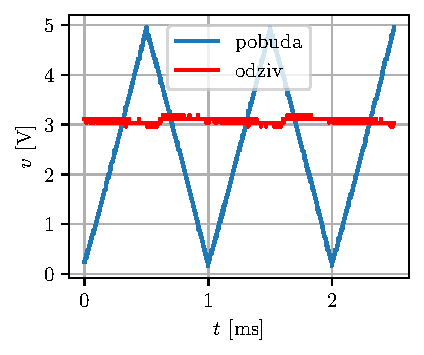
\includegraphics[scale=1]{fig_osc/FV1000s.pdf}
\captionof{figure}{Odziv konvertora na pobudu konstante frekvencije.}
\label{FV1000s}
\end{minipage}\hfill
\begin{minipage}{0.45\textwidth}
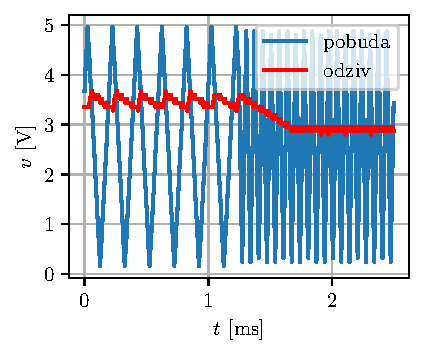
\includegraphics[scale=1]{fig_osc/FV1000d.pdf} 
\captionof{figure}{Odziv konvertora na skokovitu promenu frekvencije pobudnog napona.}  
\label{FV1000d} 
\end{minipage}
\end{center}

Pošto su oscilacije reda mV, a učestanost je $1\, \rm{kHz}$, dobijeni signal je upotrebljiv kao konstantan nivo. 

Što se tiče dinamičke karakteristike pretvarača, može se primetiti da se neželjene oscilacije koje se javljaju u nekakvoj zavisnosti od frekvencije ulaznog signala, mada, pošto nam je kod dinamičke karakteristike bitni nivoi signala na različitim učestanostima, male oscilacije ne predstavljaju veliki problem. Na slici \ref{FV1000d} je prikazano merenje dinamičke karakteristike pretvarača za signal koji se menja sa $750\, \rm{Hz}$ na $1.25\, \rm{kHz}$.


\subsubsection{Karakteristika pretvarača sa filtrom}

U prethodnoj tački se video problem sa šumom, odnosno naizmenične komponente malog signala koja potiče od pretvarača učestanosti u naponski nivo. Kada bi se pretvarač koristio sam po sebi to i ne bi predstavljalo veoma veliki problem, ali, pošto se signal sa pretvarača vodi dalje u kolu u kom postoje pojačavači, oni će pojačati taj mali signal i onda će predstavljati problem. Rešenje tog problema je filtriranje signala sa izlaza pretvarača filtrom propusnikom niskih učestanosti. Nakon filtriranja, dobiće se konstantan signal. Grafik odziva pretvarača sa filtrom propusnikom niskih učestanosti na izlazu na pobudu sa konstantnom frekvencijom je dat na slici \ref{FV1000sNF}.


\begin{center}
\begin{minipage}{0.45\textwidth}
\centering
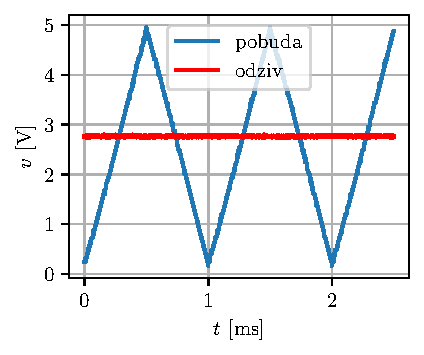
\includegraphics[scale=1]{fig_osc/FV1000sNF.pdf}
\captionof{figure}{Odziv konvertora sa filtrom na pobudu konstante frekvencije.}
\label{FV1000sNF}
\end{minipage}\hfill
\begin{minipage}{0.45\textwidth}
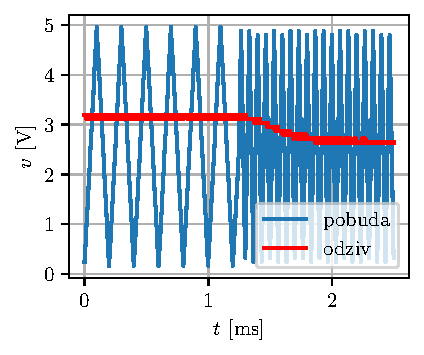
\includegraphics[scale=1]{fig_osc/FV1000dNF.pdf} 
\captionof{figure}{Odziv konvertora sa filtrom na pobudu sa promenljivom frekvencijom.}  
\label{FV1000dNF} 
\end{minipage}
\end{center}


Dodavanjem filtra propusnika niskih učestanosti se smanjila naizmenična komponenta malog signala sa reda mV na red $\upmu$V, ali se i dinamika pretvarača duplo usporila. Filtar koji ne propušta velike promene signala je uklonio naizmeničnu komponentu koja je bila posledica parazita, ali je i usporio promenu velikog signala, odnosno usporio dinamiku. Dinamička karakteristika modifikovanog pretvarača je prikazana na slici \ref{FV1000dNF}. Snaga šuma je nakon stavljanja filtra duplo smanjena. Filtar je smanjio snagu šuma na izlazu duplo, što je i prikazano na slici \ref{preklopljeni}.

\begin{figure}[h!]
    \centering
    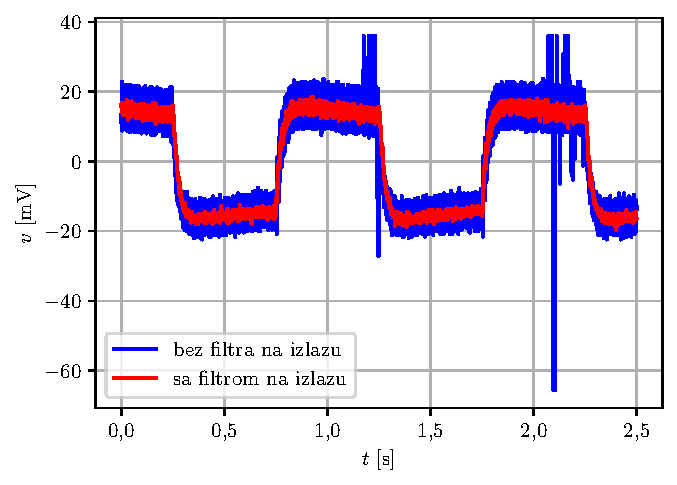
\includegraphics[scale=1]{fig_osc/filtar_preklopljen.pdf}
    \caption{Vremenski dijagram signala na izlazu konvertora frekvencije u napon bez i sa filtrom na izlazu.}
    \label{preklopljeni}
\end{figure}


Pošto se za kontrolni signal dovodi izlaz generatora signala koji predstavlja pozitivnu unipolarnu povorku pravougaonih impulsa, radi lakšeg upravljanja je optimalnije dovesti signal čiji je nivo srazmeran brzini motora. 

Karakteristika pretvarača sa i bez filtra je više manje ista zato što filtar ne menja funkciju pretvarača nego samo filtrira komponente na većim učestanostima, dok pretvarač sam po sebi ima  veliko slabljenje na većim učestanostima, tako da dodavanje filtra ne predstavlja problem u tom smislu. Izmerena karakteristika pretvarača je data na slici \ref{FVkka}.

\begin{figure}[h!]
    \centering
    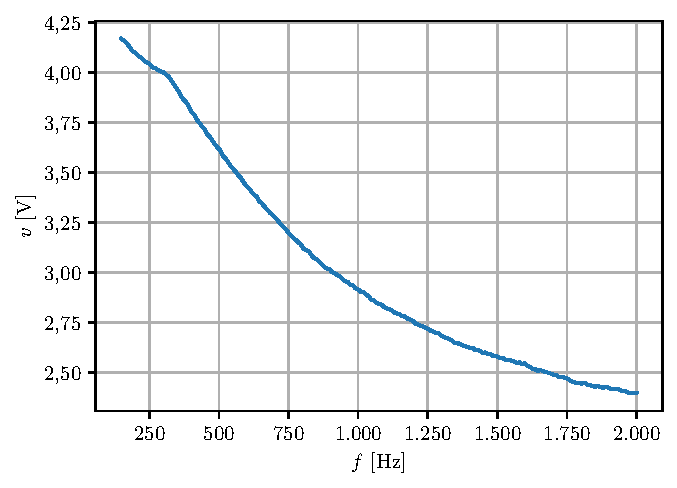
\includegraphics[scale=1]{fig_osc/FVkka.pdf}
    \caption{Prenosna karakteristika pretvarača učestanosti.}
    \label{FVkka}
\end{figure}



\subsection{Merenje karakteristika pojačavača snage}
\subsubsection{Statička prenosna karakteristika}

Kao što je već pomenuto u delu \ref{s:PAB} i \ref{s:PAAB}, kod pojačavača u klasi B se javlja \textit{crossover} izobličenje, i ono je izmereno i prikazano na slici \ref{PABs}. Uz modifikaciju pojačavača u klasi B, odnosno dodavanjem dioda, dobija se pojačavač u klasi AB koji nema izobličenja i ima linearnu prenosnu karakteristiku. Izmerena karakteristika pojačavača u klasi AB je data na slici \ref{PAABs}.



\begin{center}
\begin{minipage}{0.45\textwidth}
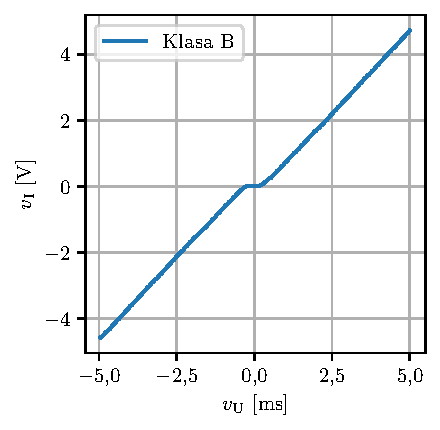
\includegraphics[scale=1]{fig_osc/PABs.pdf}
\captionof{figure}{Izmerena statička karakteristika pojačavača u klasi B.}
\label{PABs}
\end{minipage}\hfill
\begin{minipage}{0.45\textwidth}
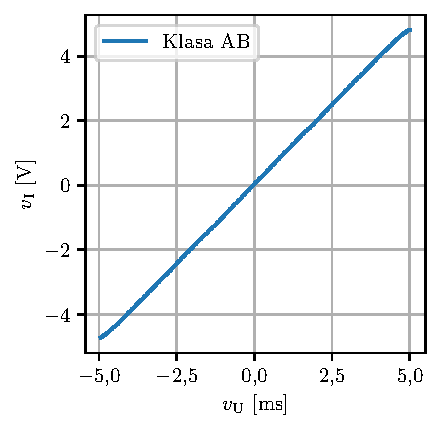
\includegraphics[scale=1]{fig_osc/PAABs.pdf} 
\captionof{figure}{Izmerena statička karakteristika pojačavača u klasi AB.}  
\label{PAABs} 
\end{minipage}
\end{center}



\subsubsection{Dinamička prenosna karakteristika sa i bez dioda}

Odskočni odziv pojačavača u klasi B je prikazan na slici \ref{PAstep}.

\begin{center}
\begin{minipage}{0.45\textwidth}
\centering
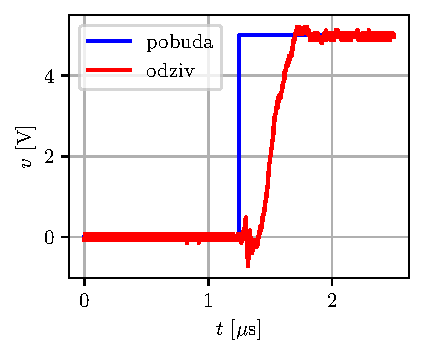
\includegraphics[scale=1]{fig_osc/PAstep.pdf}
\captionof{figure}{Odskočni odziv pojačavača snage.}
\label{PAstep}
\end{minipage}\hfill
\begin{minipage}{0.45\textwidth}
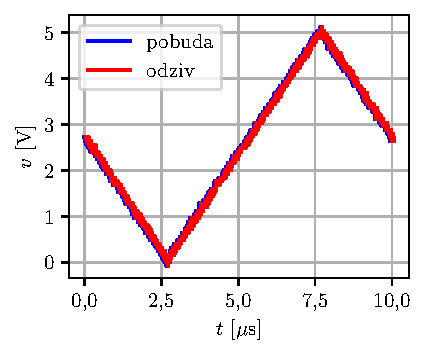
\includegraphics[scale=1]{fig_osc/PAramp.pdf} 
\captionof{figure}{Odziv pojačavača na signal rampe učestanosti $f = 100 [\rm{kHz}]$.}  
\label{PAramp} 
\end{minipage}
\end{center}


Izmerena dinamička karakteristika pojačavača u klasi B je prikazana na slici \ref{PAramp}.
Dinamika pojačavača se može još bolje videti kada se na ulazu dovede signal rampe, slika \ref{PAramp}.

Merenja pokazuju da pojačavač u klasi B prati signale čija je frekvencija reda 20kHz što je 10 puta veća učestanost od signala koji se javljaju u kolu pri ispravnom radu. Što znači da zadovoljava praktične zahteve za ispravan rad sistema. Pomenuto \textit{crossover} izobličenje ne predstavlja problem u konkretnoj praktičnoj primeni zbog prirode signala koji dolazi na ulaz pojačavača. Signal na ulazu pojačavača je učestanosti reda nekoliko kHz i rasprostranjen je po celom opsegu nivoa signala što znaci da je veoma mali interval vremena u zoni gde se javlja \textit{crossover} izobličenje, tako da praktično, ne predstavlja ozbiljan problem, i sistem može da funkcioniše ispravno. Zbog toga, je u sistemu nije neophodno da postoji pojačavač u klasi AB, a dodatno se i štedi na broju komponenti potrebnih za ispravan rad sistema.



\section{Rezultati i diskusija}



\subsubsection{Obrada rezultata merenja}
Od signala sa slike \ref{vremenski} su dobijeni ostali već pomenuti signali pomoću Python skripte koja radi na sledeći način. Pošto su podaci koji stižu binarni, ili $5 \unit{V}$ ili $0 \unit{V}$ obrada signala je podrazumevala brojanje perioda koje je bilo realizovano tako što su se brojali podaci koji su $5 \unit{V}$ počevši od prvog, zatim svi naredni podaci koji su nule sve do prvog sledećeg koji je opet $5 \unit{V}$. Na taj način imamo broj odbiraka signala u jednoj periodi, postupak se ponavlja za svaku narednu periodu. Učestanost jedne periode se računa kao $f_{\rm periode} = \frac{1}{(n-1)T_{\rm s}}$. Dobijeni broj predstavlja učestanost obrađene periode i predstavlja jednu tačku na grafiku zavisnosti periode od vremena. Postupak se ponavlja za sve periode u prikupljenim podacima. 
Mana ovakvog pristupa je povećanje greške merenja sa povećanjem učestanosti signala. Dakle, ako imamo da je $f_0 = \frac{1}{T}$, najveća greška pri očitavanju učestanosti je jedan period odabiranja $\Delta T$ što dalje dovodi do toga da je najveća greška učestanosti $\Delta f = f \frac{f \Delta T}{1 - (f \Delta T)^2}$. Procentualna greška u odnosu na frekvenciju signala se može dobiti kao: $\frac{\Delta f}{f} = \frac{f \Delta T}{1 - (f \Delta T)^2}$. Sada je već jasno da se sa povećanjem učestanosti povećava i greška pri pogrešnom računanju frekvencije, što je i prikazano na slici \ref{fGreska}.

\begin{figure}[h!]
    \centering
    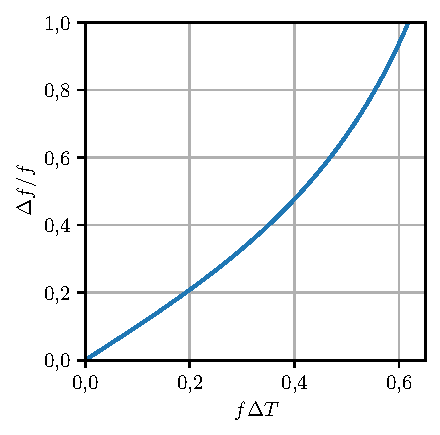
\includegraphics[scale=1]{fig_teorija/fGreska.pdf}
    \caption{Odnos normalizovane relativne greške u odnosu na normalizovanu frekvenciju.}
    \label{fGreska}
\end{figure}

\break

\subsection{Sistem sa poboljšanjima pojačavača snage}

Kao što je već objašnjeno u \ref{s:PAB} i \ref{s:PAAB}, postoji razlika između pojačavača u klasi B i pojačavača u klasi AB. Nelinearna izobličenja kod pojačavača u klasi B nisu predstavljala veliki problem dok je u sistemu korišćen P regulator sa beskonačnim pojačanjem, jer je tada signal na ulazu pojačavača snage bio izrazito oscilatornog karaktera i u veoma malim intervalima u vremenu se nalazio u zoni nelinearnosti pojačavača, što nije predstavljalo problem. Izmenama u regulatora, odnosno prelazak sa P na PI regulator signal na ulazu u pojačavač je postao manji i samim tim veći vremenski period se nalazi u zoni nelinearnih izobličenja pojačavača što je dovelo do toga se pojačavač snage poboljša, odnosno zameni pojačavačem u klasi AB koji nema nelinearna izobličenja. U ovom delu se može jasno videti tok projektovanja, odnosno modifikacije sistema koji se projektuje. Promene u jednom delu sistema potencijalno izazivaju potrebu za promenu drugog dela sistema kako bi delovi sistema bili kompatibilni i radili ispravno. Jasno je da uz menjanje delova sistema može lako doći i do promene karakteristike i osobina celog sistema. Zbog toga je bitno da se na pravilan način izaberu delovi sistema i pre svega teorijski proveriti njihov povezan rad, a onda projektovati sistem hardverski. Ovaj način projektovanja ne garantuje ispravan rad sistema odmah nakon njegovog hardverskog projektovanja, samo smanjuje greške koje se mogu predvideti i pre hardverskog projektovanja sistema. Na ovaj način se minimizuju greške sistema u početnom stadijumu hardverskog projektovanja.

\subsection{Sistem sa poboljšanjima senzora}
Pretvarač učestanosti u napon koji je pomenut u delu \ref{sec:fvKonvertor} dobro vrši funkciju konvertovanja učestanosti signala na ulazu u napon. Problem koji ima je unošenje šuma. To samo po sebi ne bi predstavljalo veliki problem, ali zbog pojačavača u sistemu, šum može dovesti do neispravnog rada celog sistema. Zbog toga je, kao što je opisano u delu \ref{s:FVNF} dodat filtar propusnik niskih učestanosti na izlaz pretvarača i time rešen problem šuma, teorijski. Pošto filtar nije idealan, šum i dalje postoji, ali to ne predstavlja veliki problem jer je šum značajno oslabljen tako da ne predstavlja problem ostatku sistema. Kao što se vidi, pored projektovanja sistema na isti način teorijski i hardverski, rezultati se ne poklapaju u potpunosti, ali je zadržano rešenje zato što je to dovoljno dobro za ispravan rad sistema. Teorijska i hardverska implementacija, pored toga što su teorijski iste, neće dati iste rezultate u većini slučajeva, ali vrlo verovatno će se dobiti zadovoljavajući rezultati, tako da je obavezno teorijski isprojektovati sistem pre hardverskog projektovanja.

\subsection{Sistem sa promenjenim regulatorom} \label{s:sspr}


Sistem sa P regulatorom radi relativno dobro. Problem je konstantna statička greška i preveliko pojačanje koje pojačava i neželjene komponente signala, odnosno šum. Zamenom P regulatora za PI regulator je dobijen sistem koji ima konačno pojačanje i nema statičku grešku. Cena za to poboljšanje je preskok. Koeficijenti su izabrani na taj način da preskok bude što manji, a da se ujedno i zadovolji brzina odziva sistema. U sistemima upravljanja, nakon zamene PI regulatora umesto P regulatora, sledi zamena PI regulatora za PID regulator koji dodaje i diferencijator u sistem. U konkretnom slučaju to nije potrebno jer bi diferencijator pogoršao stvari, baš zbog velike nelinearnosti sistema. Konačno, jedine ideje za dalju modifikaciju datog sistema sa slike \ref{nps} su eventualne promene konstante proporcionalnosti $K_{\rm p}$ i integracione konstante $T_{\rm i}$ radi dobijanja drugačijeg oblika odziva. Razlog tome je različita upotreba sistema i drugačijih komponenti. Ako se sitem koristi za kretanje, veliki preskok i oscilacije nisu optimalne, a potrebno je imati brzinu koja se zada sistemu. Dok recimo ako se sistem koristi kao rashladni sistem, nije toliko bitno ako postoji preskok, ili oscilacije ili čak i mala greška u stacionarnom stanju. Tako da, predlozi daljih modifikacija i poboljšanja sistema se ne mogu dati jer ne postoji generalizovan slučaj nego zavisi od konkretne implementacije i načina upotrebe sistema.

Projektovanje \textit{bang-bang} regulatora, odnosno P regulatora sa beskonačnim pojačanjem je relativno jednostavno uz korišćenje operacionog pojačavača. Projektovanje PI regulatora je malo složenije jer je potrebno podesiti parametre $K_{\rm p}$ i $T_{\rm i}$ takve da zadovolje zahteve koji su postavljeni. Podešavanjem koeficijenata je potrebno da se sistem ubrza onoliko koliko dinamika sistema to dozvoljava, i da se dobije relativno mali preskok. Dodatno, potrebno je podesiti parametre na taj način da oni budu realizibilni u hardveru. Električna šema PI regulatora koja je korišćena za merenja je prikazana na slici \ref{PIreg}.

\begin{figure}[h!]
    \centering
    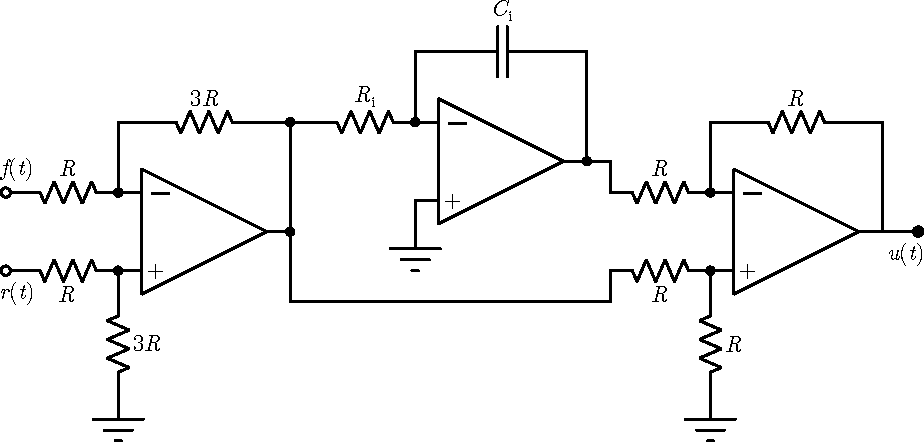
\includegraphics[scale=1]{fig/PIregEL.pdf}
    \caption{Električna šema projektovanog PI regulatora.}
    \label{PIreg}
\end{figure}

Da bi se isprojektovao PI regulator potrebno je znati prenosnu funkciju sistema $H(s) = \frac{K_{\rm m}}{T_{\rm m}s + 1}$, odnosne njene koeficijente, kao što je objašnjeno u delu \ref{s:PI}. Koeficijenti mogu varirati u zavisnosti od sistema, u konkretnom slučaju oni iznose $K_{\rm m} = 0.314$ i $T_{\rm m} = 132 \, \rm{ms}$. Koeficijenti se mogu dobiti merenjem odziva sistema $H(s)$ na nekoliko različitih pobuda i usrednjavanjem odziva sistema. Rezultati merenja i model usrednjenog odziva su dati na slici \ref{Hsrednje}.

\begin{figure}[h!]
    \centering
    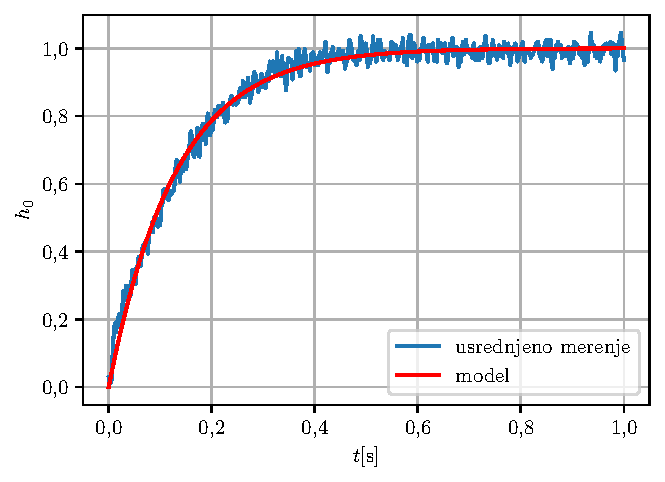
\includegraphics[scale=1]{fig_pi/Hsrednje.pdf}
    \caption{Usrednjen relativni odziv sistema $H(s)$ i njegov model.}
    \label{Hsrednje}
\end{figure}



Uz pomoć softverskog alata GNU Octave je moguće isprojektovati model regulatora za više različitih koeficijenata i dobiti teorijski očekivani odskočni odziv sistema sa projektovanim regulatorom. Projektovana su dva regulatora, jedan sa bržim odzivom i preskokom i drugi, sporiji i bez preskoka. Preklopljeni rezultati softverskog modela i merenja izlaza sistema za različite koeficijente PI regulatora su prikazani na slikama \ref{k3t100} i \ref{k3t10}.

\begin{figure}[h!]
    \centering
    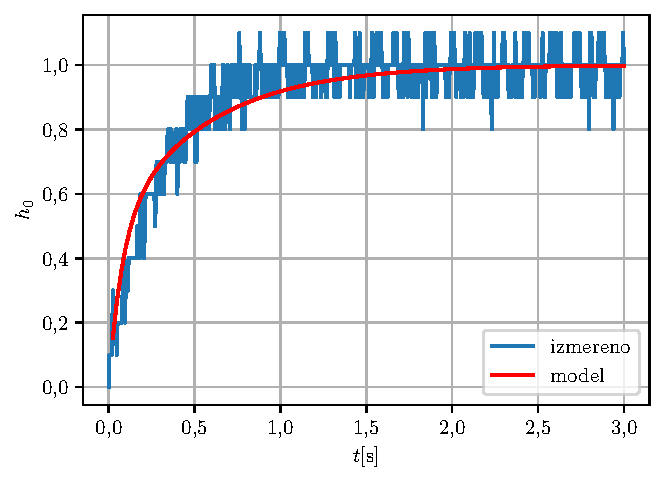
\includegraphics[scale=1]{fig_pi/k3t100.pdf}
    \caption{Odskočni odziv sistema sa parametrima PI regulatora $K_{\rm p} = 3$ i $T_{\rm i} = 10 \, \rm{ms}$.}
    \label{k3t100}
\end{figure}

\begin{figure}[h!]
    \centering
    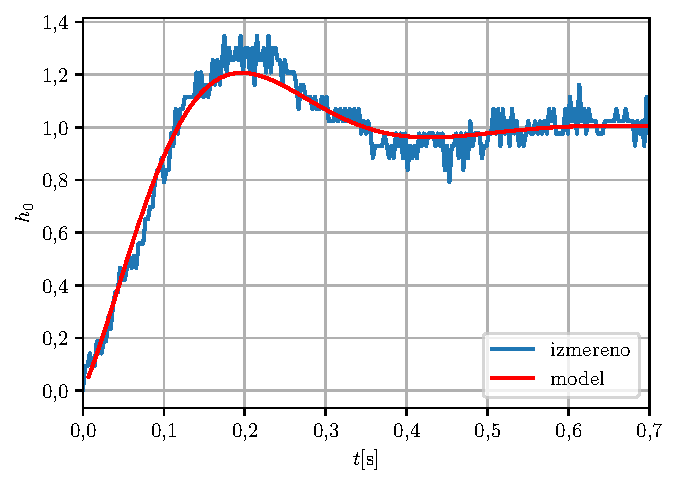
\includegraphics[scale=1]{fig_pi/k3t10.pdf}
    \caption{Odskočni odziv sistema sa parametrima PI regulatora $K_{\rm p} = 3$ i $T_{\rm i} = 100 \, \rm{ms}$.}
    \label{k3t10}
\end{figure}

\break

Na slikama \ref{Hsrednje}, \ref{k3t100} i \ref{k3t10} $h_0$ predstavlja relativnu brzinu motora.

Prenosna funkcija za sistem bez preskoka sa slike \ref{k3t100} je oblika $W(s) = \frac{7.136 s + 23.79}{s^2 + 14.71 s + 23.79}$. Dva pola funkcije su $-12.86$ i $-1.85$, nula funkcije je $-3.33$. Polovi i nule date prenosne funkcije su prikazani na slici \ref{zplane1}. Prenosna funkcija za sistem sa preskokom sa slike \ref{k3t10} oblika $W(s) = \frac{7.136 s + 237.9}{s^2 + 14.71 s + 237.9}$. Dva pola funkcije su $-7.36 + j13.56$ i $-7.36 - j13.56$, nula funkcije je $-33.34$. Polovi i nule date prenosne funkcije su prikazani na slici \ref{zplane2}. \cite{dos}

\begin{center}
\begin{minipage}{0.45\textwidth}
\centering
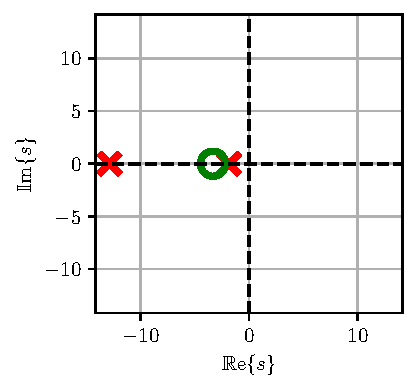
\includegraphics[scale=1]{fig_zplane/BezPreskok.pdf}
\captionof{figure}{Polovi i nule prenosne funkcije za sistem bez preskoka.}
\label{zplane1}
\end{minipage}\hfill
\begin{minipage}{0.45\textwidth}
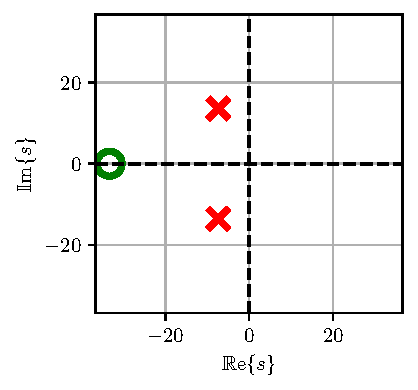
\includegraphics[scale=1]{fig_zplane/Preskok.pdf} 
\captionof{figure}{Polovi i nule prenosne funkcije za sistem sa preskokom.}  
\label{zplane2} 
\end{minipage}
\end{center}

Na slici \ref{zplane1} su prikazani polovi i nule prenosne funkcije bez preskoka. Za karakteristike sistema su bitnije pozicije polova od pozicija nula. Ako se polovi nalaze na realnoj osi, sistem nema oscilacija i odziv sistema na odskočnu pobudu se nakon nekog vremena ustaljuje, što su polovi dalji od imaginarne ose to se odziv sistema brže ustali dok u slučaju kada su polovi bliži imaginarnoj osi odziv sistema se sporije ustali. Što se tiče slike \ref{zplane2}, odnosno u slučaju konjugovano kompleksnih polova sa leve strane imaginarne ose, odziv sistema ima oscilacije koje se s vremenom priguše. Amplituda oscilacija zavisi od imaginarnog dela polova, dok njihova učestanost zavisi od udaljenost od imaginarne ose, odnosno što su konjugovano kompleksni polovi dalji od imaginarne ose to je frekvencija oscilacija veća. \cite{octave}



\subsection{Nelinearna ograničenja sistema}

Šum je jedan od najvećih problema u sistemu. Naime, u sistemu postoje pojačavači koji treba da pojačaju mali signal kako bi mogla da se vrši njegova dalja hardverska obrada, ali pošto su ti signali već sami po sebi relativno mali, potrebno je da pojačanja budu velika. Problem nastaje kada se tu javi šum koji prolazi kroz pojačavač s velikim pojačanjem i samim tim pojačava šum do značajnijih nivoa koji stvaraju velika neliearna ograničenja. Ovaj problem se može donekle rešiti filtriranjem i modifikacijama sistema na taj način da se mogu smanjiti pojačanja pojačavača. To je jedan od razloga zbog kojeg se nakon P regulatora sa beskonačnim pojačanjem uveo PI regulator koj ima konačno pojačanje. Dodatno, kao što je napomenuto u delu \ref{s:PI}, integrator teorijski smanjuje grešku u stacionarnom stanju na nulu. Realno to nije slučaj, ali greška je toliko mala da je nemerljiva, tako da, u konkretnom slučaju može da se smatra da je nula.
\cite{osc} 
\cite{gen} 
\cite{arduino}
\cite{coolTerm}



\break

\section{Zaključak}

U ovom radu je izložen postupak projektovanja analognog sistema automatskog upravljanja motora jednosmerne struje. Ideja je bila da se uz pomoć analognog signala na ulazu sistema kontroliše brzina motora jednosmerne struje uz minimalnu grešku i što brži odziv sistema. Isprojektovan je hardver koji je sačinjen od pojačavača snage, motora jednosmerne struje i konvertora učestanosti u napon. Dobijanje boljih rezultata je postignuto modifikacijama sistema, prvenstveno filtriranjem. Odrađena su sva potrebna merenja i ustanovljeno je da sistem daje teorijski očekivane rezultate što je i pokazano u delu \ref{s:sspr}, na slikama \ref{k3t100} i \ref{k3t10}.

Moguća optimizacija ovog rada je zamena motora motorom koji ima bolju dinamiku i uz povećanje napona napajanja, i dodavanjem hlađenja na tranzistorima, radi postizanja većih brzina. Ideja za dalji rad na projektu je uzimanje u obzir smer okretanja osovine motora koji se može realizovati uz korišćenje dve diode kao što je prikazano na slici \ref{enc}. Prate se pojavljivanja uzlaznih ivica signala A i B, i u zavisnosti od toga koji se prvi pojavio se jednoznačno može odrediti smer okretanja osovine motora. Još jedna ideja je da se za ulazni signal koriste prijemnik i predajnik i na taj način je moguće omogućiti kontrolu brzine motora na daljinu.

Isprojektovani analogni sistem automatskog upravljanja pokazuje da se teorijska rešenja podudaraju sa dobijenim izmerenim rezultatima. Dodatno, isprojektovan je sistem za kontrolu brzine motora koji ima dosta mogućnosti za modifikacije i dalje olakšavanje upravljanjem.


\break 


\begin{thebibliography}{9}

\bibitem{ems}
Vladimir Rajović, Predavanja iz predmeta Elektronski merni sistemi,
dostupno na \url{http://tnt.etf.rs/~oe4ems/Predavanja.html}, 
poslednji put pristupljeno \today

\bibitem{fiz}
Predrag Marinković, Fizika 1 Skripta,
Beograd, oktobar, 2017.

\bibitem{mit}
Yen-Jie Lee, Predavanja iz predmeta Fizika 3, oscilacije i talasi,
dostupno na \url{https://ocw.mit.edu/courses/8-03sc-physics-iii-vibrations-and-waves-fall-2016/pages/part-i-mechanical-vibrations-and-waves/lecture-1/}, 
poslednji put pristupljeno \today

\bibitem{arduino}
Microchip Arduino Mega 2560, Datasheet,
dostupno na \url{https://content.arduino.cc/assets/ATmega640-1280-1281-2560-2561-Datasheet-DS40002211A.pdf}, 
poslednji put pristupljeno \today

\bibitem{dos}
Vladimir Petrović, Digitalna Obrada Signala,
dostupno na \url{http://tnt.etf.rs/~19e043dos/vezbe.php},
poslednji put pristuljeno \today

\bibitem{oe}
Radivoje Đurić, materijali za predmet Osnovi Elektronike,
dostupno na \url{http://oe2oe.etf.bg.ac.rs/},
poslednji put pristupljeno \today

\bibitem{encArduino}
Članak na temu "\textit{How rotary encoder works and interface it with Arduino}",
dostupno na \url{https://lastminuteengineers.com/rotary-encoder-arduino-tutorial/},
poslednji put pristupljeno \today

\bibitem{coolTerm}
Dokumentacija za softver "\textit{CoolTerm}",
dostupno na \url{https://freeware.the-meiers.org/CoolTerm_ReadMe.txt.html},
poslednji put pristupljeno \today



\end{thebibliography}




\end{document}



